\documentclass[ABNT, FAPESP]{zentera}

\department{Faculdade de Engenharia elétrica e de computação}
\institution{Universidade Estadual de Campinas}
\supervisor{Marcos Julio Rider Flores}
\author{Lucas Zenichi Terada}
\title{Reconfiguração das redes de distribuição de energia elétrica operando em diferentes níveis de demanda}
\date{\today}
\numberwithin{equation}{section}

\usepackage{tikz,lipsum,lmodern}


\begin{document}

\makecover
%\maketitle

\begin{abstract}

\end{abstract}
\thispagestyle{empty}
\clearpage
\listoffigures
\thispagestyle{empty}
\clearpage
\listoftables
\thispagestyle{empty}
\clearpage
%Lista de nomenclaturas
\makenomenclature
\renewcommand{\nomname}{Lista de símbolos e nomenclaturas}
\renewcommand\nomgroup[1]{%
  \item[\bfseries
  \ifstrequal{#1}{C}{Conjuntos}{%
  \ifstrequal{#1}{V}{Variáveis}{%
  \ifstrequal{#1}{P}{Parâmetros}{
  \ifstrequal{#1}{A}{Abreviações}{}}}}%
]}

\nomenclature[A]{AMPL}{A Modeling Language for Mathematical Programming}
\nomenclature[A]{ANEEL}{Agência nacional de energia elétrica}
\nomenclature[A]{KNITRO}{Nonlinear Interior-point Trust Region Optimizer}
\nomenclature[A]{SDEE}{Sistema de distribuição de energia elétrica}
\nomenclature[A]{RSD}{Reconfiguração do sistema de distribuição}
\nomenclature[A]{PL}{Programação Linear}
\nomenclature[A]{PNL}{Programação não linear}
\nomenclature[A]{PLIM}{Programação linear inteiro misto}
\nomenclature[A]{PNLIM}{Programação não linear inteiro misto}
\nomenclature[A]{PCSOIM}{Programação cônica de segunda ordem inteiro misto}
\nomenclature[A]{Bonmin}{Basic Open-source Nonlinear Mixed INteger programming}

\nomenclature[C]{$\Omega_b$}{Conjunto de nós do sistema}
\nomenclature[C]{$\Omega_l$}{Conjunto de circuitos do sistema}
\nomenclature[C]{$\Omega_{ch}$}{Conjunto de chaves do sistema}

%\nomenclature[P]{$ $}{}
\nomenclature[P]{$R_{ij}$}{Resistência entre o no nó i e o nó j}
\nomenclature[P]{$X_{ij}$}{Reatância entre o nó i e o nó j}
\nomenclature[P]{$Z_{ij}$}{Impedância entre o nó i e o nó j}
\nomenclature[P]{$P_i^D$}{Demanda de potência ativa no nó i}
\nomenclature[P]{$Q_i^D$}{Demanda de potência reativa no nó i}
%\nomenclature[P]{$P_j^D$}{Demanda de potência ativa no nó j}
%\nomenclature[P]{$Q_j^D$}{Demanda de potência reativa no nó j}
%\nomenclature[P]{$P_k^D$}{Demanda de potência ativa no nó k}
%\nomenclature[P]{$Q_k^D$}{Demanda de potência reativa no nó k}
\nomenclature[P]{$P_i^S$}{Potência ativa fornecida pela subestação no nó i}
\nomenclature[P]{$P_i^S$}{Potência reativa fornecida pela subestação no nó i}
%\nomenclature[P]{$P_j^S$}{Potência ativa fornecida pela subestação no nó j}
%\nomenclature[P]{$P_j^S$}{Potência reativa fornecida pela subestação no nó j}
%\nomenclature[P]{$P_k^S$}{Potência ativa fornecida pela subestação no nó k}
%\nomenclature[P]{$P_k^S$}{Potência reativa fornecida pela subestação no nó k}
\nomenclature[P]{$\underline{V}$}{Limite mínimo de tensão permitido}
\nomenclature[P]{$\overline{V}$}{Limite máximo de tensão permitido}
\nomenclature[P]{$\overline{I}_{ij}$}{Limite máximo de fluxo de corrente entre os nós i e j}
\nomenclature[P]{$\overline{I}_{ij}^{ch}$}{Fluxo de corrente máximo permitido na chave entre o nó i e o nó j}



%\nomenclature[V]{$ $}{}
\nomenclature[V]{$V_i$}{Magnitude da tensão no nó i}
\nomenclature[V]{$V_j$}{Magnitude da tensão no nó j}
\nomenclature[V]{$V_k$}{Magnitude da tensão no nó k}
\nomenclature[V]{$\Vec{V}_i$}{Fasor tensão no nó i}
\nomenclature[V]{$\Vec{V}_j$}{Fasor tensão no nó j}
\nomenclature[V]{$\Vec{V}_k$}{Fasor tensão no nó k}
\nomenclature[V]{$I_{ij}$}{Magnitude da corrente entre o nó i e o nó j}
\nomenclature[V]{$I_{ki}$}{Magnitude da corrente entre o nó k e o nó i}
\nomenclature[V]{$\vec{I}_{ij}$}{Fasor corrente entre o nó i e o nó j}
\nomenclature[V]{$\vec{I}_{ki}$}{Fasor corrente entre o nó k e o nó i}
\nomenclature[V]{$V_i^{sqr}$}{Variável que representa o quadrado da tensão $V_i$}  
\nomenclature[V]{$V_j^{sqr}$}{Variável que representa o quadrado da tensão $V_j$}
\nomenclature[V]{$V_k^{sqr}$}{Variável que representa o quadrado da tensão $V_k$}
\nomenclature[V]{$P_{ij}$}{Fluxo de potência ativa entre o nó i e o nó j}
%\nomenclature[V]{$P_{ki}$}{Fluxo de potência ativa entre o nó k e o nó i}
%\nomenclature[V]{$P_{ji}$}{Fluxo de potência ativa entre o nó j e o nó i}
\nomenclature[V]{$Q_{ji}$}{Fluxo de potência reativa entre o nó j e o nó i}
%\nomenclature[V]{$Q_{ij}$}{Fluxo de potência reativa entre o nó i e o nó j}
%\nomenclature[V]{$Q_{ki}$}{Fluxo de potência reativa entre o nó k e o nó i}
\nomenclature[V]{$P_{ij}^{ch}$}{Fluxo de potência ativa na chave entre o nó i e o nó j}
\nomenclature[V]{$Q_{ij}^{ch}$}{Fluxo de potência reativa na chave entre o nó i e o nó j}
\nomenclature[V]{$w_{ij}$}{Variável binária que representa o estado da chave entre o nó i e o nó j}


\printnomenclature

\tableofcontents
\thispagestyle{empty}
\clearpage
\section{Introdução}

Os sistemas de distribuição de energia elétrica (SDEE) são planejados como redes de malhas interconectadas. Com a finalidade de operar de forma mais eficiente de modo a coordenar a proteção do sistema mais facilmente e reduzir a corrente de curto circuito, o SDEE opera com uma topologia radial \cite{Romais2014ReconfiguracaoMista}.

Os SDEE devem operar de forma a respeitar tanto as restrições de carga quanto as restrições operacionais. Dado que o sistema está operando em regime permanente é interessante operá-lo em estado de mínimas perdas. Para isso reconfigura-se o sistema de distribuição de modo a reduzir as perdas ôhmicas ao longo da rede.

O problema de reconfiguração do sistema de distribuição (RSD) é um problema de planejamento da operação das chaves alocadas ao longo dos alimentadores e consiste na abertura e/ou fechamento das chaves com o objetivo de melhorar um índice de desempenho.

A reconfiguração ótima é uma importante ferramenta para aumentar a confiabilidade de um SDEE, especialmente quando a automação avançada e tecnologias de redes inteligentes (smartgrids) tornam-se mais importantes e mais acessíveis às concessionarias de distribuição.

Os benefícios de se reduzir as perdas de potência ativa no sistema de distribuição são:% 

\begin{itemize}
    \item Alívio do sistema de distribuição: com a redução das perdas de potência ativa, o sistema é aliviado, o que leva a uma maior vida útil dos equipamentos, uma maior capacidade de fornecimento e um melhor perfil da magnitude de tensão no sistema;

    \item Adiamento de investimentos para a expansão do sistema de distribuição: a redução das perdas de potência tem como consequência a redução dos fluxos de potência nos condutores, e desta forma é adiada a necessidade de reforços na rede.
    
    \item Melhoria na qualidade de energia: a reconfiguração melhora o perfil da magnitude de tensão do sistema;
    
    \item Adiamento da necessidade de ampliação da capacidade de transmissão: a rede de distribuição pode reduzir o carregamento de linhas de transmissão no horário de pico, aumentando efetivamente a capacidade de transmissão;
    
    \item Adiamento da ampliação da capacidade de geração: menos unidades de geração operando são necessárias no horário de pico;
    
    \item Redução do uso de combustíveis: ao reduzir as perdas, reduz-se a necessidade de geração de energia a partir de fontes não renováveis, o que leva a uma economia no uso de combustíveis fósseis;
    
    \item Benefícios ambientais: a redução no uso de combustíveis fósseis tem como consequência a redução de poluição;
    
    \item Redução na contratação de energia elétrica para grandes clientes: ao reduzir as perdas das redes dos grandes clientes, reduz-se o consumo de energia elétrica.
\end{itemize}

A reconfiguração do sistema de distribuição é um problema de otimização cuja modelagem matemática pode ser classificada das seguintes formas, como descrito em \cite{Goncalves2013ModelosRadiais}:

\begin{itemize}
    \item PL: Programação Linear
    
    \item PNL: Programação não linear
    
    \item PLIM: Programação linear inteiro misto
    
    \item PNLIM: Programação não linear inteiro misto
    
    \item PCSOIM: Programação cônica de segunda ordem inteiro misto
\end{itemize}

% Para solucionar esses problemas utilizam-se de ``solvers'' que são programas cuja finalidade é encontrar uma solução ótima para um problema de programação.

Problemas de PL podem ser resolvidos usando algoritmos convencionais como simplex e pontos interiores.
Já para problemas de PNL existem diversas técnicas como método de Newton e relaxação Lagrangeana.
Problemas de PLIM podem ser resolvidos usando técnicas baseadas em \emph{branch and bound}.
Problemas de PNLIM são complicados de serem solucionados e imagina-se que solvers comerciais usem algoritmos baseados em \emph{branch and bound}. 

O problema de RSD, como será visto, é um problema não linear inteiro misto.
Problemas não lineares são complicados de serem solucionados devido à dificuldade de convergência dos algoritmos usados para determinar soluções ótimas. 
Além disso, em problemas de PL e PLIM existem condições necessárias e suficientes de otimização teoricamente provadas que garantem se uma dada solução é factível ou não.
Já para problemas PNL e PNLIM não existem tais condições. Por outro lado existem as heurísticas e meta-heurísticas que buscam resolver esses problemas de forma a buscar uma solução satisfatória em tempo adequado \cite{Goncalves2013ModelosRadiais}.  

Alguns trabalhos relevantes na literatura que abordam a reconfiguração de redes radiais com demandas fixas foram tratados em \cite{Baran1989NetworkBalancing} abordando algoritmos heurísticos.
Algoritmos genéticos como mostrado em  \cite{Souza2015AlgoritmoVariaveis} se mostraram interessantes para resolver problemas de característica não linear.
Em \cite{deCastro2002AnOptimization} mostra-se uma interessante abordagem que simula o comportamento do sistema imunológico do corpo humano para solucionar um problema de otimização não linear.
Outra abordagem interessante é a transformação de um problema PNLIM em um problema PCSOIM (programação cônica de segunda ordem inteiro misto) através do relaxamento de uma restrição do problema como mostra \cite{Romais2014ReconfiguracaoMista}.
\section{Objetivos}

A fim de reduzir as perdas ôhmicas ao longo da rede, este projeto tem o objetivo de propor um método para determinar uma nova topologia de modo a redistribuir o fluxo de corrente entre os ramos do SDEE.

Para isso o método deve seguir os seguintes requisitos:

\begin{itemize}
    \item A nova topologia deve ser radial;
    
    \item As restrições operativas devem ser respeitadas na nova topologia.
\end{itemize}

Por fim, será descrito como se equacionam as leis que regem o SDEE bem como os limites em que as grandezas físicas devem estar contidas.

\section{Metodologia}

O modelo para reconfiguração do sistema de distribuição de energia elétrica, abordado nesse projeto, foi implementado em linguagem de modelagem matemática com o objetivo de otimizar um sistema.

\subsection{Otimização}

Otimização é o estudo de problemas nos quais procuram-se minimizar ou maximizar funções dentro de um conjunto de valores factíveis para o mesmo.

É difícil fornecer uma ``taxonomia'' de otimização porque muitos dos subcampos possuem vários links. Na figura~\ref{fig:taxonomia} é exibida uma perspectiva, focada principalmente nos subcampos de otimização determinística com uma única função objetivo~\cite{neosguidetaxonomia}.

\begin{figure}[H]
    \centering
    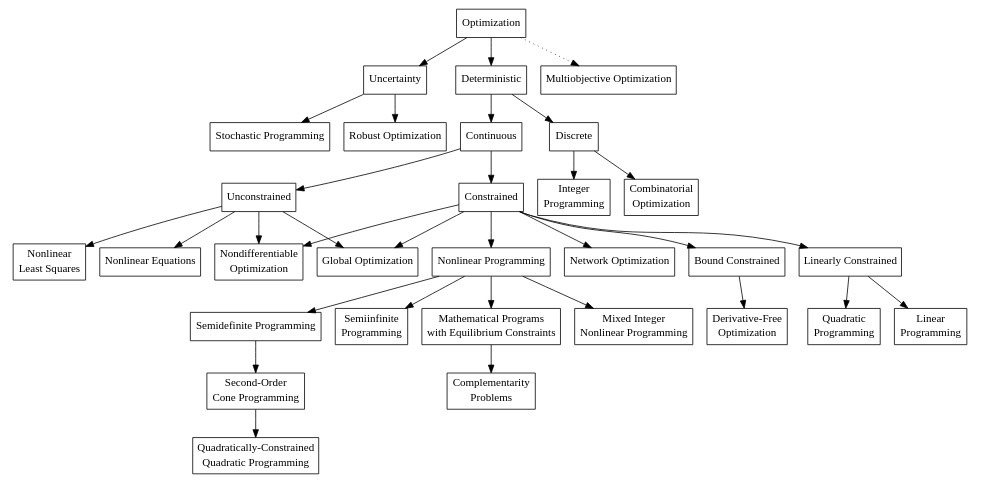
\includegraphics[width = \textwidth]{3_Methodology/otim.jpeg}
    \caption{``Taxonomia'' para problemas de otimização (fonte: ~\cite{neosguidetaxonomia})}
    \label{fig:taxonomia}
\end{figure}

\subsection{Introdução a Linguagem de Programação Matemática}

Linguagens de programação matemática são programas capazes de modelar interpretar o modelo matemático em um arquivo capaz de ser lido por \emph{solvers}, softwares com algoritmos para resolver problemas de otimização.

A sintaxe de uma linguagem de modelagem matemática é muito semelhante a modelagem algébrica, realizada de modo genérico é possível estender o modelo desenvolvido para outros problemas.

Os benefícios envolvendo o uso da linguagem estão relacionados ao fato de ser possível lidar com modelos algébricos, complexos e de larga escala, de maneira fácil e intuitiva que serão traduzidos em dados que podem ser processados por programas solucionadores.

Exemplos de problemas como descritos em \cite{Fourer2003AMPLProgramming} são:

\begin{itemize}
    \item Modelo de transporte \emph{multicommodity};
    
    \item Modelo de produção multiperiódico;
    
    \item Modelo de produção e transporte.
\end{itemize}

Os exemplos citados anteriormente são apenas uma parcela de uma infinidade de problemas de programação de larga escala.

A vantagem desse arranjo é que o mesmo modelo algébrico pode ser usado para resolver um problema de mesma natureza mas de tamanho diferente.

\subsection{AMPL}

O AMPL é uma linguagem procedural de modelagem algébrica cuja função é descrever e resolver problemas a partir do seu modelo matemático. 
A linguagem fora desenvolvida nos \emph{Bell Labs} por Robert Fourer, David Gay e Brian Kernighan com o intuito de ajudar as pessoas a comunicar modelos de otimização para sistemas de computação, aproveitando o poder e a conveniência de formulações algébricas familiares \cite{ampl}. 

Possui, atualmente, suporte para uma grande diversidade de \textit{solvers} tanto comerciais quanto código aberto.

A estrutura básica de um modelo em AMPL é da seguinte forma como mostrada em \cite{taha2008pesquisa}:

\begin{table}[H]
    \centering
    \caption{Estrutura de um modelo em AMPL}
    \begin{tabular}{|c|l|}
        \hline
        \multirow{4}{*}{Representação algébrica} & Definição dos conjuntos\\ & Definição dos parâmetros\\ & Definição das variáveis\\ & Representação do modelo\\ \hline
        \multirow{3}{*}{Implementação do modelo} & Dados de entrada\\ & Solução do modelo\\ & Apresentação dos resultados\\
        \hline
    \end{tabular}
    \label{tab:estrut_AMPL}
\end{table}

\subsection{Julia JuMP}

JuMP é uma linguagem de modelagem específica de domínio para otimização matemática incorporada em Julia~\cite{DunningHuchetteLubin2017}.
JuMP foi escrito puramente em Julia e possui código aberto, possuindo suporte para diversos \emph{solvers}, tanto comerciais quanto de código aberto.

Julia é uma linguagem de programação voltada para computação científica do tipo dinâmica criada no MIT.
A proposta da linguagem é suprir a falta de alta performance que geralmente acompanha as linguagens de dinâmicas.

De modo geral a linguagem Julia combina a velocidade de processamento semelhante a linguagens estáticas com os artifícios de linguagens dinâmicas tais como \emph{Python} e MATLAB.

\subsection{\emph{Solvers}}

\emph{Solvers}, como dito anteriormente, são programas que tem como finalidade buscar uma solução ótima baseada em um conjunto de parâmetros e podem ser tanto comerciais quanto constituídos de código aberto.
Ambas as categorias podem resolver determinados problemas de acordo com a natureza do sistema.


Um exemplo de \emph{solver} usado para resolver problemas de otimização linear e quadrática em variáveis contínuas e inteiras é o CEPLEX, \emph{solver} comercial baseado essencialmente em linguagem C cuja licença pertence à empresa IBM.
O suporte é fornecido para soluções de problemas quadráticos convexos, não convexos e restrições quadráticas convexas \cite{amplCEPLEX}. Os algoritmos usados são:

\begin{itemize}
    \item Problemas contínuos: primal e dual simplex, ponto interior;
    
    \item Problemas de números inteiros: \textit{branch and bound}, heurísticas de viabilidade e geradores de corte.
\end{itemize}

Outro exemplo de \emph{solver}, esse utilizado para solução de problemas de otimização não lineares, é o KNITRO.
O KNITRO é um pacote de programas em C para resolver otimização não linear e não linear inteiro misto, uma particularidade do software foi a grande atenção dada ao desempenho dos algoritmos KNITRO em classes mais simples de problemas, como sistemas de equações não-lineares e problemas irrestritos, uma vez que essas tarefas são cruciais na solução de problemas de programação não linear \cite{Byrd2006Knitro:Optimization}.
Segundo a Artelys, empresa responsável pelo software, o mesmo conta com os seguintes recursos para a solução de problemas de otimização, mostrados em \cite{knitroweb}:

\begin{itemize}
    \item Quatro algoritmos de ponto ativo/conjunto interno para problemas PNL;
    
    \item Três algoritmos para otimização discretas de problemas PNLIM;
    
    \item restrições de complementaridade para problemas de equilíbrio.
\end{itemize}

A entrada de um \emph{solver} para solução de problemas PNLIM, pode ser tomado como exemplo o manual disponível no NEOS-server como mostrado em \cite{neosguide}.

\begin{tcolorbox}[colback=white!10,title =\textbf{Dados de entrada de um \emph{solver}}]
    \begin{minipage}{\dimexpr\textwidth-\shadowsize-2\fboxrule-2\fboxsep-8pt}
    
    \begin{center}
        Min: $f(x,y)$   
    \end{center}

    \hspace{2cm}Sujeito a: 

    \begin{align*}
        c_{i}(x,y) = 0 \qquad \forall i&\in E\\
        c_{i}(x,y) \leq 0 \qquad \forall i&\in I\\
        x \qquad &\in X\\
        y \qquad &\in Y \quad \text{inteiro}
    \end{align*}
    \end{minipage}
    
    \vspace{1cm}
    
    Onde cada $c_{i}(x,y)$ é um mapeamento de $R^n \to R$, e $E$ e $I$ são conjuntos de índices para restrições de igualdades e desigualdades respectivamente. Tipicamente, as funções $f$ e $c_{i}$ têm algumas propriedades de suavidade, isto é, uma ou duas vezes continuamente diferenciáveis.
\end{tcolorbox}

\subsection{Hipóteses e definições da formulação do problema}

\begin{figure}[H]
    \centering
    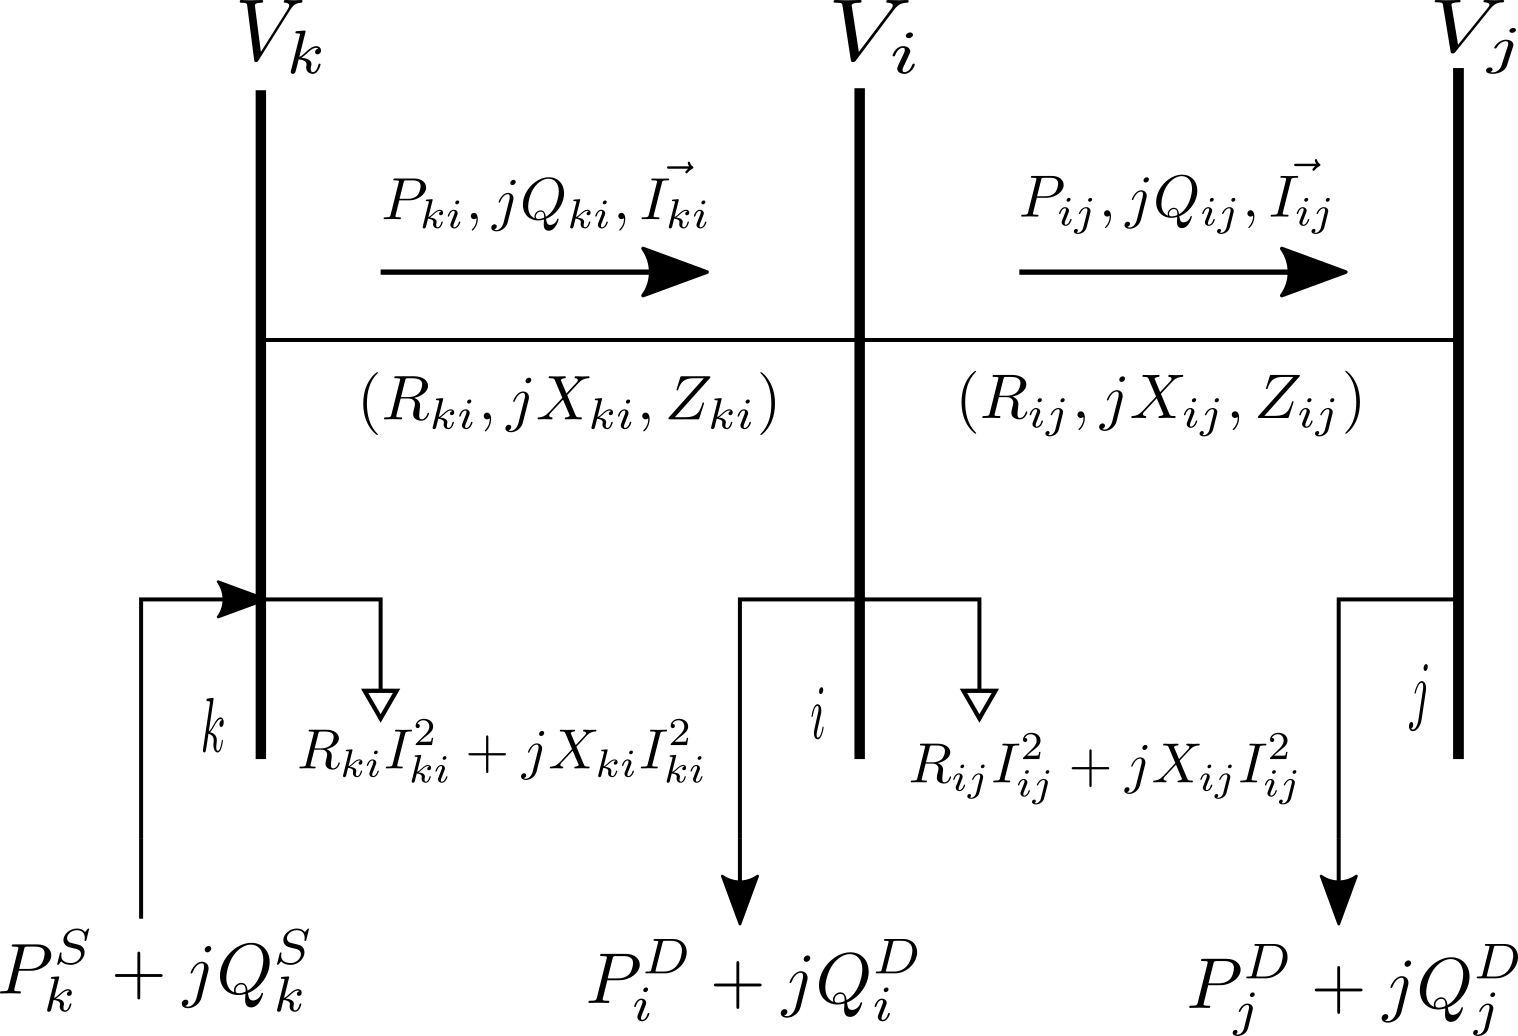
\includegraphics[width=0.7\textwidth]{3_Methodology/diagrama_nos.png}:
    \caption{Sistema de distribuição (Representação em barras)}
    \label{fig:SDR}
\end{figure}

Hipóteses adotadas:
Visando representar o funcionamento em regime permanente de um sistema de distribuição de energia, são feitas as seguintes hipóteses (comumente usadas nas formulações de varredura de fluxo de carga \cite{Shirmohammadi1988ANetworks} e mostradas na figura \ref{fig:SDR}):

\begin{itemize}
    \item As demandas das cargas na rede de distribuição são representadas como potência ativa e reativas constantes;

    \item O sistema é balanceado e representado pelo seu equivalente monofásico;
    
    \item As perdas de potência ativa e reativa no circuito \textit{ij} estão concentradas no nó \textit{i};
    
    \item As chaves são representadas como curtos circuitos de impedância nula.
\end{itemize}

\subsection{Modelo de otimização}

O modelo de otimização para RSD interpretado pelo AMPL possui a seguinte forma:

\begin{tcolorbox}[colback=white!10,title =\textbf{Modelo de um problema de otimização para RDS}]
    \begin{minipage}{\dimexpr\textwidth-\shadowsize-2\fboxrule-2\fboxsep-8pt}
    
    \begin{center}
        Minimizar: Função objetivo        
    \end{center}

    \hspace{2cm}Sujeito a:

    \begin{center}
        Restrições físicas\\
        Restrições operativas\\
    \end{center}
    \end{minipage}
\end{tcolorbox}


As restrições do problema devem ser tais que modelem as leis da física que regem um sistema de distribuição de energia elétrica e as faixas com as quais essas grandezas podem operar ao longo da rede.
Para isso define-se dois conjuntos de restrições, restrições físicas e restrições operativas.
\section{Modelagem do problema}

O problema de RSD envolve restrições não lineares e variáveis quadráticas, a fim de, em um primeiro momento, realizar uma tentativa de linearização e simplificação do problema, propõe-se uma mudança de variável que será aplicado nas equações ao longo deste documento.

\begin{align}
    I_{ij}^{sqr} = I_{ij}^{2}\;\forall ij \in \Omega_l \text{ e } V_{i}^{sqr} = V_{i}^{2}\; \forall i\in\Omega_b 
    \label{eq:change_variable}
\end{align}

%Explicar o significado de conjunto de circuitos e conjunto de nós do sistema


\subsection{Função objetivo}

Dado o modelo de otimização a ser interpretado pela linguagem de modelagem, é possível definir a função objetivo com base na figura~\ref{fig:SDR}.
A fim de reduzir as perdas ôhmicas na rede elétrica, a função objetivo do problema consiste em minimizar a somatória das perdas por resistência elétrica no conjunto de circuitos do sistema.

Definindo $c^{lss}$ como parâmetro que representa o custo das perdas de potência ativa na rede têm-se:

\begin{equation}
    \begin{split}
        \text{Min} = & c^{lss}\sum_{ij\in\Omega_{l}}R_{ij}I_{ij}^{2}\\
        = & c^{lss}\sum_{ij\in\Omega_{l}}R_{ij}I_{ij}^{sqr}
    \end{split}
    \label{eq:funcobjetivo}
\end{equation}

Tal que $\Omega_{l}$ é o conjunto de circuitos do sistema.
\subsection{Balanço de potência}

\begin{figure}[H]
    \centering
    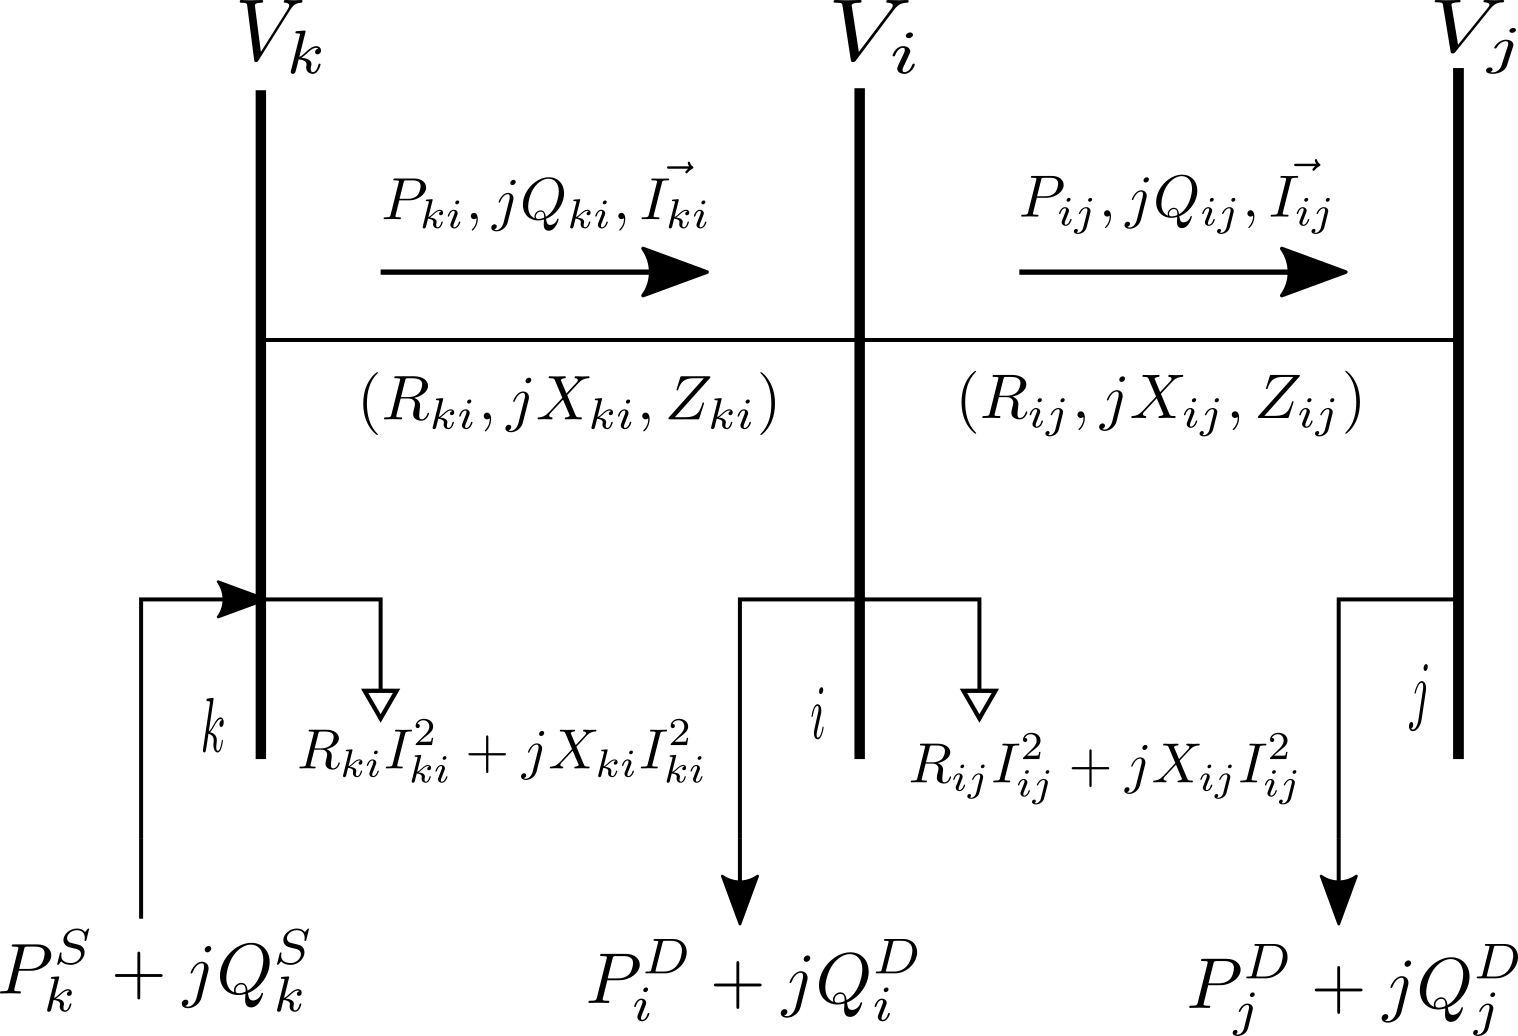
\includegraphics[width=0.6\textwidth]{3_Methodology/diagrama_nos.png}
    \caption{Exemplo de um diagrama de balanço de potência entre nós de um sistema de distribuição de energia elétrica}
    \label{fig:balanco_pot}
\end{figure}

A figura~\ref{fig:balanco_pot} representa a forma expandida da figura~\ref{fig:SDR}, para melhor compreensão do problema de balanço de potência, onde $m$ e $n$ representam um número qualquer de nós ligados ao nó $i$. 
Para isso considere que nos parâmetros e variáveis que representam um ramo, o primeiro subíndice representa o nó de partida e o segundo subíndice representa o nó de chegada (exemplo: $P_{12}$ se refere ao fluxo de potência ativa que vai do nó 1 para o nó 2).

Seja $P_{i}^{D}$ e $Q_{i}^{D}$ potência ativa e reativa demandada no nó i respectivamente e $P_{i}^{S}$ e $Q_{i}^{S}$ potência ativa e reativa gerada no nó $i$ respectivamente, têm-se que:

\begin{equation*}
    \sum_{ki\in\Omega_{l}}P_{ki} - \sum_{ij\in\Omega_{l}}(P_{ij} + R_{ij}I_{ij}^{2}) + P_{i}^{S} = P_{i}^{D}\quad\forall i \in\Omega_{b}
\end{equation*}

\begin{equation*}
    \sum_{ki\in\Omega_{l}}Q_{ki} - \sum_{ij\in\Omega_{l}}(Q_{ij} + X_{ij}I_{ij}^{2}) + Q_{i}^{S} = Q_{i}^{D}\quad\forall i \in\Omega_{b}
\end{equation*}

Dado que $\Omega_{b}$ é o conjunto de nós do sistema.
É possível mudar a variável \textit{k} pela variável \textit{j}, uma vez que ambas pertencem ao conjunto $\Omega_{l}$ e os somatórios envolvendo-as estão desconectadas, desse modo:
%desconectadas -> desconectados (para concordar com "somatórios")

\begin{equation}
    \sum_{ji\in\Omega_{l}}P_{ji} - \sum_{ij\in\Omega_{l}}(P_{ij} + R_{ij}I_{ij}^{2}) + P_{i}^{S} = P_{i}^{D}\quad\forall i \in\Omega_{b}\label{eq:fluxo_pot_ativa}  
\end{equation}


\begin{equation}
    \sum_{ji\in\Omega_{l}}Q_{ji} - \sum_{ij\in\Omega_{l}}(Q_{ij} + X_{ij}I_{ij}^{2}) + Q_{i}^{S} = P_{i}^{D}\quad\forall i \in\Omega_{b}\label{eq:fluxo_pot_reativa}
\end{equation}

O sistema de equações não lineares em \ref{eq:fluxo_pot_ativa} e \ref{eq:fluxo_pot_reativa} representam a operação em regime permanente de uma rede elétrica radial e são frequentemente utilizados no método de varredura de fluxo de carga \cite{Shirmohammadi1988ANetworks} e \cite{Cespedes1990NewNetworks}.
\subsection{Queda de tensão entre nós}


O conjunto de equações a seguir mostram o caso típico de formulação do problema de fluxo de carga para redes elétricas radiais.

Da figura \ref{fig:SDR}, a queda de tensão do circuito é definida pela equação \ref{eq:queda_tensao}.

\begin{equation}
    \Vec{V}_{i} - \Vec{V}_{j} = I_{ij}(R_{ij} + jX_{ij})\quad\forall i,j \in \Omega_{l}
    \label{eq:queda_tensao}
\end{equation}

Em que $\Omega_{l}$ é o conjunto de circuitos, ou seja, o conjunto de todos os nós do sistema.

Através da fórmula para o cálculo da potência aparente, $I_{ij}$ pode ser calculado usando a equação \ref{eq:corrente_ramo}.

\begin{equation}
    I_{ij} = \left(\frac{P_{ij} + jQ_{ij}}{\Vec{Vj}}\right)^{*}\quad\forall ij \in \Omega_{l}
    \label{eq:corrente_ramo}
\end{equation}

Substituindo $I_{ij}$ da equação \ref{eq:corrente_ramo} na equação \ref{eq:queda_tensao} obtém-se a equação \ref{eq:queda_tensao_pot} que define a queda de tensão em função das potências e impedâncias do circuito.


Seja $(P_{ij} + jQ_{ij})^{*} = (P_{ij} - jQ_{ij})$, logo:

\begin{equation}
    (\Vec{V}_{i} - \Vec{V}_{j})\Vec{V}_{j}^{*} = (P_{ij} - jQ_{ij})(R_{ij} + jX_{ij}) \quad\forall ij \in \Omega_{l}
    \label{eq:queda_tensao_pot}
\end{equation}

Considerando que $\Vec{V}_{i} = V_{i}\angle{\theta_{i}}$, $\Vec{V}_{j} = V_{j}\angle{\theta_{j}}$ e $\theta_{ij} = \theta_{i} - \theta_{j}$, tal que  $V_{i}$ e $V_{j}$ representam as magnitudes da tensão em seus respectivos nós bem como $\theta_{i}$ e $\theta_{j}$ representam seus ângulos.
Dessa forma a equação \ref{eq:queda_tensao_pot} pode ser escrita decompondo a fase de suas exponenciais, como mostra a equação \ref{eq:queda_tensao_sencos}.

\begin{equation}\label{eq:queda_tensao_sencos}
    V_{i}V_{j}[cos\theta_{ij} + jsen\theta_{ij}] - V_{j}^{2} = (P_{ij} - jQ_{ij})(R_{ij} + jX_{ij}) \quad\forall ij \in \Omega_{l}
\end{equation}

Identificando as partes real e imaginária na equação \ref{eq:queda_tensao_sencos}, obtém-se:

\begin{equation}
    V_{i}V_{j}cos\theta_{ij} = V_{j}^{2} + (R_{ij}P_{ij} + X_{ij}Q_{ij})\quad\forall ij \in \Omega_{l}
    \label{eq:queda_tensao_real}
\end{equation}

\begin{equation}
    V_{i}V_{j}sen\theta_{ij} = X_{ij}P_{ij} - R_{ij}Q_{ij}\quad\forall ij \in \Omega_{l}
    \label{eq:queda_tensao_imaginaria}
\end{equation}

Usando a fórmula da trigonometria, que é a relação básica entre o seno e o cosseno, $sen^{2}(\theta_{ij}) + cos^{2}(\theta_{ij}) = 1$, e somando os quadrados das equações \ref{eq:queda_tensao_real} e \ref{eq:queda_tensao_imaginaria}, obtém-se:

\begin{equation}
    V_{i}^{2} - 2(R_{ij}P_{ij} + X_{ij}Q_{ij}) - Z_{ij}^{2}I_{ij}^{2} - V_{j}^{2} = 0\quad\forall ij \in \Omega_{l}
    \label{eq:queda_tensao_restricao}
\end{equation}

Nota-se que a equação \ref{eq:queda_tensao_restricao} não depende da diferença angular entre as tensões, e é possível obter a magnitude da tensão do nó ($V_j$) em termos da magnitude inicial ($V_i$), o fluxo de potência ativa ($P_{ij}$), o fluxo de potência reativa ($Q_{ij}$), a magnitude do fluxo de corrente ($I_{ij}$) e os parâmetros elétricos do ramo \textit{ij}.

\subsection{Fluxo de corrente em um ramo}

Na equação de queda de tensão, a magnitude do fluxo de corrente $I_{ij}$ é mostrada na equação \ref{eq:corrente_magnitude}, calculada a partir do produto com seu complexo conjugado.

\begin{equation}
    I_{ij}^{2} = \frac{P_{ij}^{2}+Q_{ij}^{2}}{V_{j}^{2}}\quad\forall ij \in \Omega_{l}
    \label{eq:corrente_magnitude}
\end{equation}

\subsection{Restrições operativas do sistema}

O problema de reconfiguração está sujeita a restrições operativas imposta pela agência reguladora, tais como limite de tensão, correntes tanto para o conjunto de ramos do sistema quanto para a operação das chaves.
Dessa forma é possível determinar as restrições operativas para o funcionamento do SDEE.

\subsubsection{Limites de tensão}

Em um sistema de distribuição de energia elétrica é preciso garantir que a tensão em um nó esteja dentro de uma faixa de operação determinada por norma, por isso uma restrição fundamental para o problema é a restrição de limites de tensão em um nó, determinada pela seguinte equação:

\begin{equation}
    \underline{V}^{2} \leq V_{i}^{sqr} \leq \overline{V}^{2}\qquad\forall i \in\Omega_{b}
\end{equation}

Onde $\underline{V}$ e $\overline{V}$ representam o limite inferior e superior de tensão, respectivamente, que uma rede pode possuir.


\subsubsection{Limite de corrente}

Assim como as tensões, o fluxo de corrente também deve ser limitado para não comprometer o SDEE.
Assim a equação que descreve a restrição é:

\begin{equation}
    0 \leq I_{ij}^{sqr} \leq \overline{I}_{ij}^{2} \qquad\forall ij\in\Omega_{l} 
\end{equation}

\subsubsection{Chaves presentes no sistema}

Para reconfiguração do SDEE, existem chaves ao longo da rede que podem ser modificadas de modo a garantir a operação desejada.
Considere as seguintes restrições:

\begin{figure}[H]
    \centering
    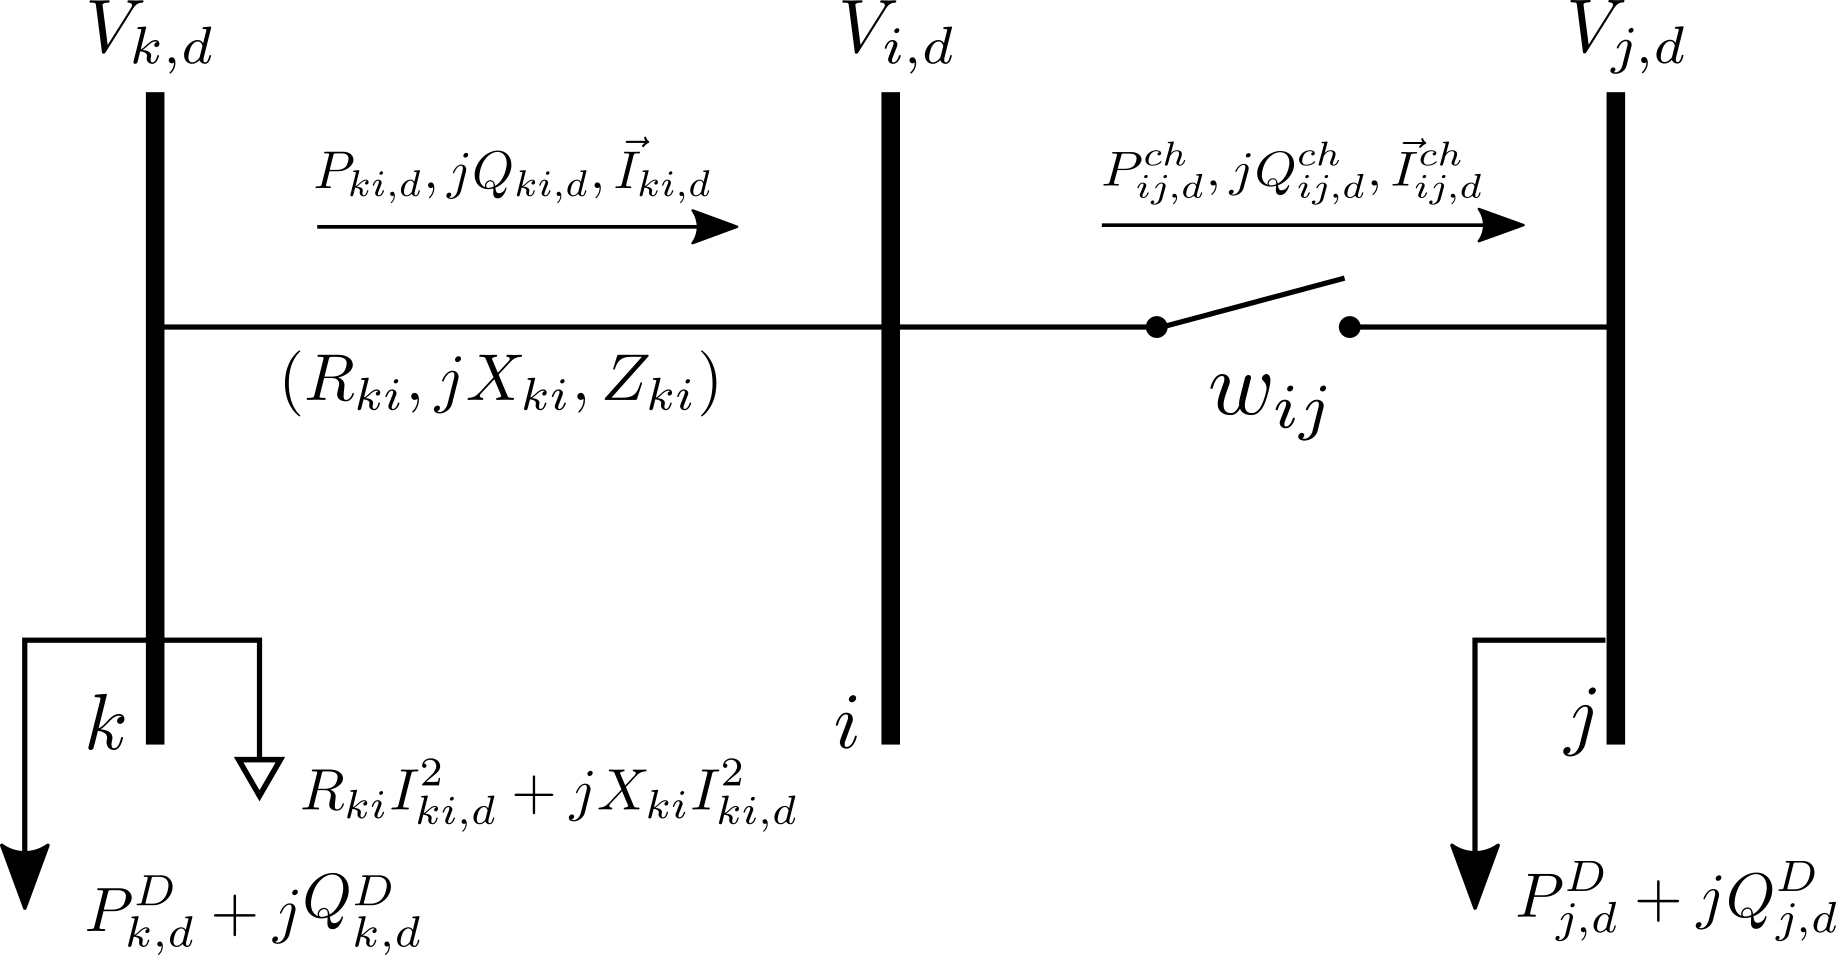
\includegraphics[scale = 1.3]{4_Modeling/diagrama_chaves.png}
    \caption{Modelo de uma chave conectada entre dois nós}
    \label{fig:diagrama_chave}
\end{figure}
    
\begin{itemize}
    \item Balanço de potência
\end{itemize}
    Com base na figura \eqref{fig:diagrama_chave}, faz-se necessário reformular as equações de balanço de potência, expressas em~\eqref{eq:fluxo_pot_ativa} e \eqref{eq:fluxo_pot_reativa}, adicionando as variáveis que representam as chaves na modelagem do problema.

\begin{equation}
    \sum_{ji\in\Omega_{l}}P_{ji} - \sum_{ij\in\Omega_{l}}(P_{ij} + R_{ij}I_{ij}^{sqr})+ \sum_{ji\in\Omega_{ch}}P_{ji}^{ch} -\sum_{ij\in\Omega_{ch}}P_{ij}^{ch} + P_{i}^{S} = P_{i}^{D}\quad\forall i \in\Omega_{b}\label{eq:fluxo_pot_ativa_chaves}  
\end{equation}
    
    
\begin{equation}
    \sum_{ji\in\Omega_{l}}Q_{ji} - \sum_{ij\in\Omega_{l}}(Q_{ij} + X_{ij}I_{ij}^{sqr})+ \sum_{ji\in\Omega_{ch}}Q_{ji}^{ch} -\sum_{ij\in\Omega_{ch}}Q_{ij}^{ch} + Q_{i}^{S} = P_{i}^{D}\quad\forall i \in\Omega_{b}
    \label{eq:fluxo_pot_reativa_chaves}
\end{equation}
    
Onde $\Omega_{ch}$ representa o conjunto de chaves da rede elétrica e $w_{ij}$ é uma variável binária que representa o estado da chave \textit{ij}: se $w_{ij} = 1$ a chave ij está fechada, caso contrário a chave está aberta, ver figura~\ref{fig:diagrama_chave}. $P_{ij}^{ch}$ e $Q_{ij}^{ch}$ representam o fluxo de potência ativa e reativa da chave \textit{ij}.

As restrições expressas nas equações \eqref{eq:fluxo_pot_ativa_chaves} e \eqref{eq:fluxo_pot_reativa_chaves} são extensões das equações \eqref{eq:fluxo_pot_ativa} e \eqref{eq:fluxo_pot_reativa}, considerando a presença de chaves na rede elétrica.
    
Além do balanço de potência, outras restrições devem ser estabelecidas devido à presença de chaves, são elas:

\begin{itemize}
    \item Diferença de tensões entre dois nós conectados por uma chave
\end{itemize}

    
A diferença de tensão entre nós, na presença de chaves, deve ser igual a zero, uma vez que, de acordo com as hipóteses adotadas, a impedância da chaves é representada como uma impedância nula.
Sendo assim, usando a variável binária $w_{ij}$ é possível equacionar a restrição da seguinte forma:

\begin{equation}
    -(\overline{V}^{2} - \underline{V}^{2})(1-w_{ij}) \leq V_{i}^{sqr} - V_{j}^{sqr} \leq (\overline{V}^{2} - \underline{V}^{2})(1-w_{ij})\qquad\forall ij\in\Omega_{ch}
\end{equation}
    
É possível observar que se $w_{ij}$ for igual a 1 (chave fechada), a diferença entre as tensões no nó $i$ e nó $j$ será igual a zero, o que condiz a hipótese adotada.

\begin{itemize}
   \item Fluxo de potência na chave
\end{itemize} 
    
O fluxo de potência na chave é determinada pelas equações abaixo.
    
\begin{equation}
    -(\overline{V}\,\overline{I}_{ij}^{ch})w_{ij} \leq P_{ij}^{ch} \leq (\overline{V}\,\overline{I}_{ij}^{ch})w_{ij}\qquad\forall ij\in\Omega_{ch}   
\end{equation}
    
    
\begin{equation}
    -(\overline{V}\,\overline{I}_{ij}^{ch})w_{ij} \leq Q_{ij}^{ch} \leq (\overline{V}\,\overline{I}_{ij}^{ch})w_{ij}\qquad\forall ij\in\Omega_{ch}   
\end{equation}
    
É possível notar que se a variável $w_{ij}$ for igual a 0 (chave aberta), o fluxo de potência na chave é igual a zero, o que condiz com a proposta do elemento de circuito na rede; quando igual a 1, as restrições representam o fluxo máximo de potência ativa e reativa permitida na chave quando está energizada.

\subsubsection{Restrição de radialidade}

A representação de um SDEE é feita através de nós e circuitos. Fazendo analogia com a teoria de grafos, um SDEE pode ser considerado como um grafo formado por n arcos e m nós.
Da teoria de grafos, uma árvore é um grafo conexo sem ciclos, assim é possível comparar a topologia radial de um SDEE com uma árvore.
Como mostrado em \cite{Bazaraa1990LinearFlows}, a árvore de um grafo é um sub-grafo com ($m-1$) arcos.

Assim, pode-se dizer que a topologia de um SDEE com $n_{b}$ nós é radial se satisfaz as duas seguintes condições: Condição 1: a solução deve apresentar ($n_{b}$) circuitos; e Condição 2: a solução deve gerar uma topologia conexa. Observa-se que a restrição de radialidade tem que ser formada pelas condições 1 e 2.
Somente a condição 1 não garante a radialidade do SDEE. 

O problema de RSD cumpre com as seguintes características: 1) apenas uma única subestação existente no SDEE (nó da subestação); 2) todos os outros nós são nós de carga; 3) a primeira lei de kirchhoff, deve ser cumprida, e 4) o objetivo é encontrar a melhor topologia radial. 
A condição 1 é satisfeita pela seguinte restrição:

\begin{equation}
    |\Omega_{l}| + \sum_{ij\in\Omega_{ch}}w_{ij} = |\Omega_{b}| - 1
    \label{eq:radialidade}
\end{equation}

Em que $|\Omega|$ é um operador que calcula o número de elementos do conjunto $\Omega$.

Uma solução que satisfaz a restrição de balanço de potência (primeira Lei de Kirchhoff) tem de fornecer a demanda de potência em cada nó de carga de modo que exista um caminho entre a subestação e os nós de carga. Portanto, cada nó está ligado com a subestação, formando um grafo conexo, o que comprova a Condição 2. 
Assim, quando as restrições de balanço de potência são combinadas com a Condição 1, cada nó de carga está ligado por um único caminho com a subestação, isto é, o SDEE é conexo, sem malhas.

\begin{figure}[H]
    \centering
    
\includegraphics[scale = 0.8]{4_Modeling/restricao_fail.png}
    \caption{Exemplo de rede não radial que obedece a equação \eqref{eq:radialidade}}
    \label{fig:radialidade_wrong}
\end{figure}

Observa-se que a figura \ref{fig:radialidade_wrong}, embora respeite a equação \eqref{eq:radialidade} (5 ramos para 6 nós), não é uma topologia radial. Isso pode acontecer se e somente se a equação~\eqref{eq:radialidade} for levada em consideração.

\begin{figure}[H]
    \centering
    
\includegraphics[scale=0.6]{4_Modeling/restricao_radialidade.png}
    \caption{Exemplo de rede radial que obedece a equação \eqref{eq:radialidade}}
    \label{fig:radialidade_right}
\end{figure}

Observe agora a figura \ref{fig:radialidade_right}, note que ela é uma topologia radial, como dito anteriormente é necessário duas condições para garantir tal configuração, como no problema já existem equações que garantem a primeira Lei de Kirchhoff, a topologia final será radial. 
É possível notar que todos os nós estão interligados, direto e não direto, com o nó 1 (nó da subestação).
Isso acontece pois as equações de balanço de potência obrigam que haja fluxo de potência para atender as demandas dos mesmos.

Assim a equação \eqref{eq:radialidade} junto com \eqref{eq:fluxo_pot_ativa_chaves} e \eqref{eq:fluxo_pot_reativa_chaves} fornecem as condições necessárias para e suficientes para garantir uma topologia final radial \cite{Lavorato2012ImposingProblems}.


\section{Formulação dos problemas de programação}

Como dito anteriormente, este trabalho tem como objetivo analisar o problema de RSD como um problema de otimização.
As equações já descritas são suficientes para descrever o problema e, em conjunto, formam um problema de programação não linear (como mostra a seção seguinte) que posteriormente foram convertida em problemas de outras naturezas.
\subsection{Problema de programação não linear}

Utilizando a metodologia descrita anteriormente, é possível modelar o problema de reconfiguração de redes radiais, utilizando as equações~\ref{eq:funcobjetivo}, \ref{eq:fluxo_pot_ativa_chaves}, \ref{eq:fluxo_pot_reativa_chaves}, \ref{eq:corrente_ramo} da seguinte forma:


\begin{tcolorbox}[enhanced jigsaw,breakable,pad at break*=1mm,colback=white!10,title =\textbf{Problema de PLIM para RSD}]

\begin{align*}\label{eq:NL_funcobj}
    \text{Min}\quad c^{lss}\sum_{ij\in\Omega_l}R_{ij}I_{ij}^{sqr}
\end{align*}

Sujeito a:

\begin{equation*}\label{eq:NL_PA}
    \sum_{ji\in\Omega_{l}}P_{ji} - \sum_{ij\in\Omega_{l}}(P_{ij} + R_{ij}I_{ij}^{sqr})+ \sum_{ji\in\Omega_{ch}}P_{ji}^{ch} -\sum_{ij\in\Omega_{ch}}P_{ij}^{ch} + P_{i}^{S} = P_{i}^{D}\quad\forall i \in\Omega_{b}  
\end{equation*}

\begin{equation*}\label{eq:NL_PR}
    \sum_{ji\in\Omega_{l}}Q_{ji} - \sum_{ij\in\Omega_{l}}(Q_{ij} + X_{ij}I_{ij}^{sqr})+ \sum_{ji\in\Omega_{ch}}Q_{ji}^{ch} -\sum_{ij\in\Omega_{ch}}Q_{ij}^{ch} + Q_{i}^{S} = Q_{i}^{D}\quad\forall i \in\Omega_{b}
\end{equation*}

\begin{equation*}\label{eq:NL_voltage}
    V_{i}^{sqr} - 2(R_{ij}P_{ij} + X_{ij}Q_{ij}) - Z_{ij}^{2}I_{ij}^{sqr} - V_{j}^{sqr} = 0\quad\forall ij \in \Omega_{l}
\end{equation*}

\begin{equation*}\label{eq:NL_power}
    V_{j}^{sqr}I_{ij}^{sqr} = P_{ij}^{2}+Q_{ij}^{2}\quad\forall ij \in \Omega_{l}
\end{equation*}

\begin{equation*}\label{eq:NL_voltagekeys}
    -(\overline{V}^{2} - \underline{V}^{2})(1-w_{ij}) \leq V_{i}^{sqr} - V_{j}^{sqr} \leq (\overline{V}^{2} - \underline{V}^{2})(1-w_{ij})\qquad\forall ij\in\Omega_{ch}
\end{equation*}
    
\begin{equation*}\label{eq:NL_PAkeys}
    -(\overline{V}\,\overline{I}_{ij}^{ch})w_{ij} \leq P_{ij}^{ch} \leq (\overline{V}\,\overline{I}_{ij}^{ch})w_{ij}\qquad\forall ij\in\Omega_{ch}
\end{equation*}
    
    
\begin{equation*}\label{eq:NL_PRkeys}
    -(\overline{V}\,\overline{I}_{ij}^{ch})w_{ij} \leq Q_{ij}^{ch} \leq (\overline{V}\,\overline{I}_{ij}^{ch})w_{ij}\qquad\forall ij\in\Omega_{ch}   
\end{equation*}
    
\begin{equation*}\label{eq:NL_radialidade}
    |\Omega_{l}| + \sum_{ij\in\Omega_{ch}}w_{ij} = |\Omega_{b}| - 1
\end{equation*}

\begin{equation*}\label{eq:NL_limvoltage}
    \underline{V}^{2} \leq V_{i}^{sqr} \leq \overline{V}^{2}\qquad\forall i \in\Omega_{b}
\end{equation*}

\begin{equation*}\label{eq:NL_limcurrent}
    0 \leq I_{ij}^{sqr} \leq \overline{I}_{ij}^{2} \qquad\forall ij\in\Omega_{l} 
\end{equation*}

\begin{equation*}\label{eq:NL_binario}
    w_{ij}\quad\text{binário}\qquad\forall ij \in\Omega_{ch}
\end{equation*}
\end{tcolorbox}

O problema descrito no conjunto equações destacadas é considerado um problema de programação não linear devido à presença da restrição expressa na equação~\ref{eq:NL_power}, uma vez que ela é o produto de duas variáveis que representam tensão e corrente do sistema ($V_{j}^{sqr}$ e $I_{ij}^{sqr}$) que são iguais a soma dos quadrados das variáveis que representam as potências ativas e reativas do sistema ($P_{ij}$ e $Q_{ij}$).

\subsection{Problema de programação cônica de segunda ordem}

O problema de PNLIM pode ser convertido em um problema convexo. Relaxando a restrição não linear do problema, pode-se transformar o problema de PNLIM em um problema de programação cônica de segunda ordem inteiro misto (PCSOIM).

Em~\cite{Romais2014ReconfiguracaoMista}, é possível escrever um problema de otimização cônica em um problema de programação linear, que contenha pelo menos uma restrição cônica. 
Uma restrição cônica 
\subsection{Problema de programação linear}

Utilizando algumas aproximações, o problema de programação não linear inteiro misto pode ser convertido em um problema de programação linear inteiro misto.

Inicialmente pode-se aproximar o quadrado da tensão em um nó do circuito como o quadrado da tensão nominal.
Esta simplificação é valida e com um erro de aproximação baixo, devido ao intervalo restrito da magnitude de tensão [$\underline{V}^2$,$\overline{V}^2$] e comprovado experimentalmente depois de realizar varias simulações apresentadas em~\cite{Goncalves2013ModelosRadiais} e \cite{Alves2012Alocacao-}.
Dessa forma o primeiro termo da equação~\eqref{eq:PNLIM_power} pode ser reescrita da seguinte forma:

\begin{equation}\label{eq:L_powervoltage}
    V_{j}^{2}I_{ij}^{sqr} \approx (V^{\text{nom}})^{2}I_{ij}^{sqr}\qquad\forall ij\in\Omega_{l}
\end{equation}

Da equação~\eqref{eq:L_powervoltage}, é possível perceber que não existe mais produto entre variáveis, visto que $V^{nom}$ é um parâmetro e, portanto, uma constante do problema.

O outro passo é linearizar os termos $P_{ij}^2$ e $Q_{ij}^2$, o que é possível, utilizando o método de linearização por partes como mostrado em~\cite{Goncalves2013ModelosRadiais} e \cite{Alves2012Alocacao-}.

O método de linearização por partes consiste em uma somatória de segmentos de retas a partir de blocos discretos igualmente espaçados.
A figura~\ref{fig:linearization} mostra a discretização do módulo de uma variável pelo seu quadrado.

\begin{figure}[H]
    \centering
    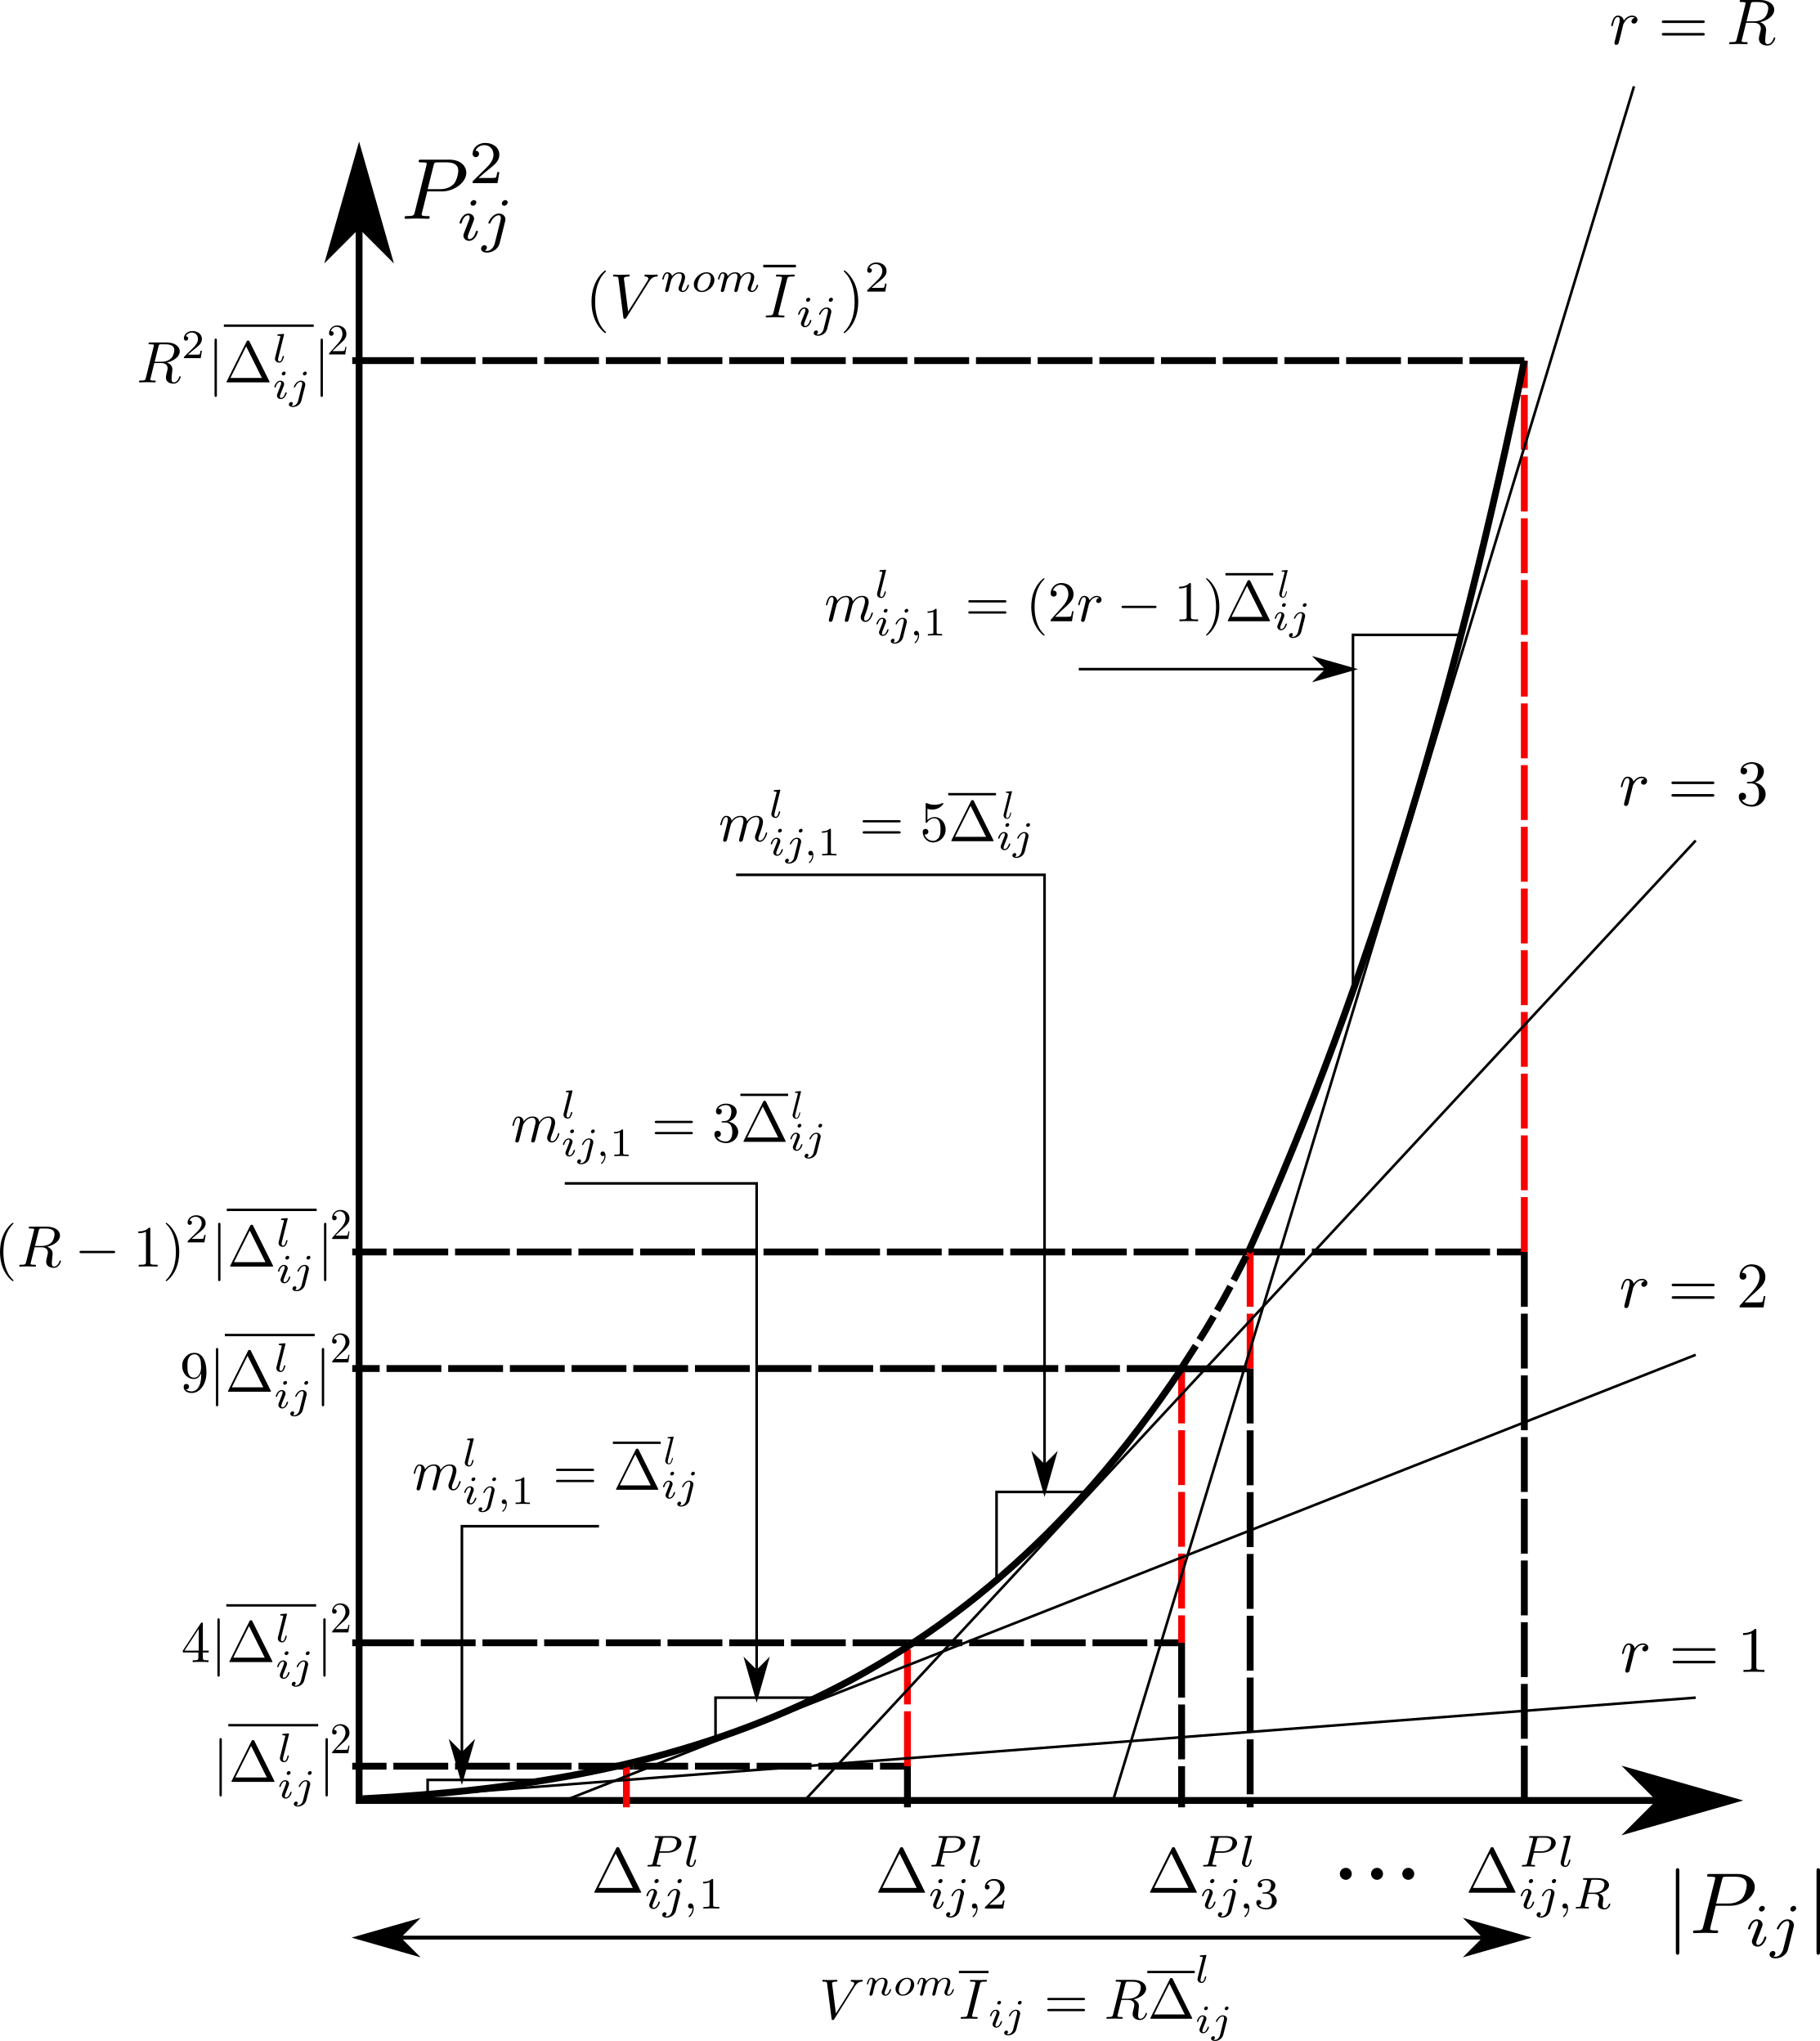
\includegraphics[width = 0.6\textwidth]{5_Formulation/lin.png}
    \caption{Linearização da potência ativa pelo método de linearização por partes}
    \label{fig:linearization}
\end{figure}{}

Com base na figura~\ref{fig:linearization}, o valor de $P_{ij}^{2}$ pode ser descrito como o somatório dos catetos paralelos ao eixo da ordenada (segmentos em vermelho), a mesma analogia pode ser feita com $Q_{ij}^{2}$, resultando na equação~\eqref{eq:Lin_quadpower}.

\begin{equation}\label{eq:Lin_quadpower}
    P_{ij}^2 + Q_{ij}^2 \approx \sum_{r = 1}^{R}m_{ij,r}^{l}\Delta_{ij,r}^{Pl} + \sum_{r = 1}^{R}m_{ij,r}^{l}\Delta_{ij,r}^{Ql} \qquad\forall ij\in\Omega_{l} 
\end{equation}

Tal que $\Delta_{ij,r}^{Pl}$ e $\Delta_{ij,r}^{Ql}$ são variáveis que representam o r-ésimo bloco de $P_{ij}$ e $Q_{ij}$ do circuito $ij$ respectivamente, as quais devem obedecer a seguinte restrição:

\begin{equation}\label{eq:Lin_Pdeltalim}
    0 \leq \Delta_{ij,r}^{Pl} \leq \overline{\Delta}_{ij,r}^l \qquad\forall ij\in\Omega_{l} 
\end{equation}

\begin{equation}\label{eq:Lin_Qdeltalim}
    0 \leq \Delta_{ij,r}^{Ql} \leq \overline{\Delta}_{ij,r}^l \qquad\forall ij\in\Omega_{l} 
\end{equation}

O parâmetro $\Delta_{ij}^{l}$ representa o valor máximo do bloco de discretização, assim dado um valor $R$ de discretizações, pode-se determinar $\Delta_{ij}^{l}$ como o quociente entre o módulo da potência aparente máxima e a quantidade de discretizações $R$, obtendo assim a equação~\eqref{eq:Lin_maxdelta}.

\begin{equation}\label{eq:Lin_maxdelta}
    \overline{\Delta}_{ij}^{l} = \frac{V^{\text{nom}}\overline{I}_{ij}}{R} \qquad\forall ij\in\Omega_{l} 
\end{equation}

$m_{ij,r}^{l}$ representa a inclinação do r-ésimo bloco de potência ativa e reativa no circuito $ij$ e é descrito pela equação~\eqref{eq:Lin_m}.

\begin{equation}\label{eq:Lin_m}
    \begin{split}
        m_{ij,r}^{l} & = \frac{r^2|\overline{\Delta_{ij}^{l}}|^2 - (r-1)^2|\overline{\Delta_{ij}^{l}}|^2}{|\overline{\Delta_{ij}^{l}}|}\qquad\forall ij\in\Omega_{l}\\
        & = |\overline{\Delta_{ij}^{l}}|(r^2 - r^2 + 2r - 1)\qquad\quad\forall ij\in\Omega_{l}\\
        & = (2r-1)\overline{\Delta_{ij}^{l}}\qquad\qquad\qquad\qquad\forall ij\in\Omega_{l}
    \end{split}
\end{equation}

Para que se possa implementar a linearização descrita pelas equações anteriores é preciso modelar o módulo das variáveis $P_{ij}$ e $Q_{ij}$. Isto pode ser feito utilizando duas variáveis positivas de tal modo que:

\begin{equation}\label{eq:Lin_PQmod}
    \begin{split}
        P_{ij} = P_{ij}^{+} - P_{ij}^{-} & \qquad\forall ij\in\Omega_{l}\\
        Q_{ij} = Q_{ij}^{+} - Q_{ij}^{-} & \qquad\forall ij\in\Omega_{l}
    \end{split}
\end{equation}

\begin{equation}
    \begin{split}
        0 \leq P_{ij}^{+} & \qquad\forall ij\in\Omega_{l}\\
        0 \leq P_{ij}^{-} & \qquad\forall ij\in\Omega_{l}\\
        0 \leq Q_{ij}^{+} & \qquad\forall ij\in\Omega_{l}\\
        0 \leq Q_{ij}^{-} & \qquad\forall ij\in\Omega_{l}
    \end{split}
\end{equation}

Aplicando o módulo em $P_{ij}$ e $Q_{ij}$, obtém-se:

\begin{equation}\label{eq:Lin_modPA}
        |P_{ij}| = P_{ij}^{+} + P_{ij}^{-} = \sum_{r = 1}^{R}\Delta_{ij,r}^{Pl}  \qquad\forall ij\in\Omega_{l}
\end{equation}

\begin{equation}\label{eq:Lin_modPR}
        |Q_{ij}| = Q_{ij}^{+} + Q_{ij}^{-} = \sum_{r = 1}^{R}\Delta_{ij,r}^{Ql}  \qquad\forall ij\in\Omega_{l}
\end{equation}

Por fim, o problema de programação linear inteiro misto pode ser descrito no seguinte formato:


\begin{tcolorbox}[breakable,pad at break*=1mm,colback=white!10,title =\textbf{Problema de PLIM para RSD}]

\begin{equation}\label{eq:plim}
\left.
    \begin{tabular}{ll}
               & Min ~\eqref{eq:PNLIM_funcobj}\\
    Sujeito a: &\eqref{eq:PNLIM_fluxoP} - \eqref{eq:PNLIM_voltage}, \eqref{eq:PNLIM_voltagekeys} - \eqref{eq:PNLIM_currentlim} \textbf{(Equações já propostas para RSD)}\\
    &\textbf{(Bloco de equações para linearização de~\eqref{eq:PNLIM_power})}\\
    &$(V^{nom})^{2}I_{ij}^{sqr} = \sum_{r = 1}^{R}m_{ij,r}^{l}\Delta_{ij,r}^{Pl} + \sum_{r = 1}^{R}m_{ij,r}^{l}\Delta_{ij,r}^{Ql} \qquad\forall ij\in\Omega_{l}$ \\
    &$P_{ij} = P_{ij}^{+} - P_{ij}^{-}\qquad\forall ij\in\Omega_{l}$\\
    &$Q_{ij} = Q_{ij}^{+} - Q_{ij}^{-}\qquad\forall ij\in\Omega_{l}$\\
    & $P_{ij}^{+} + P_{ij}^{-} = \sum_{r = 1}^{R}\Delta_{ij,r}^{Pl}  \qquad\forall ij\in\Omega_{l}$\\
    & $Q_{ij}^{+} + Q_{ij}^{-} = \sum_{r = 1}^{R}\Delta_{ij,r}^{Ql}  \qquad\forall ij\in\Omega_{l}$\\
    & $0 \leq \Delta_{ij,r}^{Pl} \leq \overline{\Delta}_{ij,r}^l \qquad\forall ij\in\Omega_{l}$\\
    & $0 \leq \Delta_{ij,r}^{Ql} \leq \overline{\Delta}_{ij,r}^l \qquad\forall ij\in\Omega_{l}$\\
    &$P_{ij}^{+}\in\mathbb{R}^{+}$, $P_{ij}^{-}\in\mathbb{R}^{+}$, $Q_{ij}^{+}\in\mathbb{R}^{+}$, $Q_{ij}^{-}\in\mathbb{R}^{+}\qquad\forall ij\in\Omega_{l}$\\
    & \textbf{(Definição de variáveis binárias)}\\
    &$w_{ij}\in\{0,1\}\qquad\forall ij\in\Omega_{l}$\\
    &\\
    Em que:&\\
    & $m_{ij,r}^{l}= (2r-1)\overline{\Delta_{ij}^{l}}\qquad\qquad\qquad\qquad\forall ij\in\Omega_{l} $\\
    & $\overline{\Delta}_{ij}^{l} = \frac{V^{\text{nom}}\overline{I}_{ij}}{R} \qquad\forall ij\in\Omega_{l}$
    \end{tabular}
\right \}
\end{equation} 
\end{tcolorbox}



\bibliographystyle{plain}               %Estilo de apresentação da bibliografia
\bibliography{references,webpage} %Arquivos de referência para importação

\end{document}
